%\documentclass[hyperref={pdfpagelabels=false},slidetop,9pt]{beamer}
\documentclass[slidetop,8pt]{beamer}
\usepackage[T1]{fontenc}
\usepackage[utf8]{inputenc}
\newcommand{\id}{54}
\newcommand{\nom}{Liaisons mécaniques}
\newcommand{\sequence}{04}
\newcommand{\num}{01}
\newcommand{\type}{TP}
\newcommand{\descrip}{Modélisation d'un solide. Comportement des liaisons mécaniques. Modéliser les mécanismes du laboratoire par un schéma cinématique, paramétré.}
\newcommand{\competences}{A3-C4: Analyse d'architecture et de comportement \\ &  Mod1-C1: Isolement d'un solide ou d'un système de solides \\ &  Mod2-C10-1: Modèle de solide indéformable \\ &  Mod2-C11: Modélisation géométrique et cinématique des mouvements entre solides indéformables \\ &  Mod2-C12: Modélisation cinématique des liaisons entre solides \\ &  Mod2-C15: Modélisation des actions mécaniques \\ &  Rés-C6: Utilisation d'un solveur ou d'un logiciel multi physique \\ &  Com1-C1: Différents descripteurs introduits dans le programme \\ &  Com2-C4: Outils de communication}
\newcommand{\nbcomp}{9}
\newcommand{\systemes}{Plateforme Stewart}
\newcommand{\systemessansaccent}{Plateforme Stewart}
\newcommand{\ilot}{2}
\newcommand{\ilotstr}{02}
\newcommand{\dossierilot}{\detokenize{Ilot_02 Plateforme Stewart}}
\newcommand{\imageun}{Plateforme}

\newcommand{\urlsysteme}{\href{https://www.costadoat.fr/systeme/57}{Ressources système}}
\newcommand{\matlabsimscape}{\href{https://github.com/Costadoat/Sciences-Ingenieur/raw/master/Systemes/Plateforme Stewart/Plateforme_Stewart_Simscape.zip}{Modèle Simscape}}
\newcommand{\solidworks}{\href{https://github.com/Costadoat/Sciences-Ingenieur/raw/master/Systemes/Plateforme Stewart/Plateforme_Stewart_Solidworks.zip}{Modèle Solidworks}}
\newcommand{\edrawings}{\href{https://github.com/Costadoat/Sciences-Ingenieur/raw/master/Systemes/Plateforme Stewart/Plateforme_Stewart.EASM}{Modèle eDrawings}}
\newcommand{\test}{Stewart_param1}
\newcommand{\testi}{Stewart_param2}
\newcommand{\testii}{Stewart_param3}
\newcommand{\testiii}{Stewart_param4}
\newcommand{\testiiii}{Stewart_euler}
\usepackage{etex}
\usepackage{tikz}
\usepackage[european]{circuitikz}
\usepackage{pgf}
\usepackage[all]{xy}
\usepackage{pgfpages}
\usepackage{graphbox}
\usepackage{pdfpages}
\usepackage[adobe-utopia]{mathdesign}
\usepackage{ifthen}
\usepackage{cancel}
\usepackage{framed}
\usepackage{subfig}
\usepackage{tabularx}
\usepackage{setspace}
\usepackage{soul}
\usepackage{schemabloc}
\usepackage{eqnarray}
\usepackage[dot, phantomtext]{dashundergaps}
\usepackage{media9}
\usepackage{multimedia}
\usepackage{textcomp}

\author{Renaud Costadoat}
\institute{Lycée Dorian}

\usepackage{multido}
\usepackage{multirow}
\usepackage{multicol} % Portions de texte en colonnes
\usepackage{flafter}%floatants après la référence

\usepackage{color}
\usepackage{xcolor}
\usepackage{colortbl}

\usepackage[gen]{eurosym}
\usepackage{tikz}
%\usepackage{pstricks,pst-node,pst-tree,pst-solides3d}
\usepackage{lmodern}
\usepackage[francais]{babel}
\usepackage{pslatex}
\usetheme{renaud}
\usepackage{times}
\usepackage{amsmath}
\usepackage{verbatim}
\usepackage{moreverb}
%\usetikzlibrary{arrows,shapes}
\usepackage{graphicx}
\usepackage{psfrag}
\usepackage{wrapfig}
\usepackage{etoolbox}

\definecolor{gris25}{gray}{0.75}
\definecolor{bleu}{RGB}{18,33,98}
\definecolor{bleuf}{RGB}{42,94,171}
\definecolor{bleuc}{RGB}{231,239,247}
\definecolor{rougef}{RGB}{185,18,27}
\definecolor{rougec}{RGB}{255,188,204}%255,230,231
\definecolor{vertf}{RGB}{103,126,82}
\definecolor{vertc}{RGB}{220,255,191}

\setlength\parindent{24pt}
\parskip 7.2pt
\parindent 8pt

\newenvironment{rem}[1][\hsize]%
{%
    \def\FrameCommand
   {%
\rotatebox{90}{\textit{\textsf{Remarque}}} 
       {\color{bleuf}\vrule width 3pt}%
       \hspace{0pt}%must no space.
       \fboxsep=\FrameSep\colorbox{bleuc}%
  }%
    \MakeFramed{\hsize#1\advance\hsize-\width\FrameRestore}%
}%
{\endMakeFramed}%


\newenvironment{savoir}[1][\hsize]%
{%
    \def\FrameCommand
    {%
\rotatebox{90}{\textit{\textsf{Savoir}}} 
        {\color{bleuf}\vrule width 3pt}%
        \hspace{0pt}%must no space.
        \fboxsep=\FrameSep\colorbox{bleuc}%
    }%
    \MakeFramed{\hsize#1\advance\hsize-\width\FrameRestore}%
}%
{\endMakeFramed}%

\newenvironment{prob}[1][\hsize]%
{%
    \def\FrameCommand%
    {%
\rotatebox{90}{\textit{\textsf{Problematique}}} 
        {\color{rougef}\vrule width 3pt}%
        \hspace{0pt}%must no space.
        \fboxsep=\FrameSep\colorbox{rougec}%
    }%
    \MakeFramed{\hsize#1\advance\hsize-\width\FrameRestore}%
}%
{\endMakeFramed}%

\newenvironment{obj}[1][\hsize]%
{%
    \def\FrameCommand%
    {%
\rotatebox{90}{\textit{\textsf{Objectif}}} 
        {\color{vertf}\vrule width 3pt}%
        \hspace{0pt}%must no space.
        \fboxsep=\FrameSep\colorbox{vertc}%
    }%
    \MakeFramed{\hsize#1\advance\hsize-\width\FrameRestore}%
}%
{\endMakeFramed}%

\newenvironment{defi}[1][\hsize]%
{%
    \def\FrameCommand%
    {%
\rotatebox{90}{\textit{\textsf{Definition}}} 
        {\color{bleuf}\vrule width 3pt}%
        \hspace{0pt}%must no space.
        \fboxsep=\FrameSep\colorbox{rougec}%
    }%
    \MakeFramed{\hsize#1\advance\hsize-\width\FrameRestore}%
}%
{\endMakeFramed}%


\newenvironment{hypo}[1][\hsize]%
{%
    \def\FrameCommand%
    {%
\rotatebox{90}{\textit{\textsf{Hypothèse\\}}} 
        {\color{bleuf}\vrule width 3pt}%
        \hspace{0pt}%must no space.
        \fboxsep=\FrameSep\colorbox{bleuc}%
    }%
    \MakeFramed{\hsize#1\advance\hsize-\width\FrameRestore}%
}%
{\endMakeFramed}%


\newenvironment{prop}[1][\hsize]%
{%
    \def\FrameCommand%
    {%
\rotatebox{90}{\textit{\textsf{Propriété}}} 
        {\color{bleuf}\vrule width 3pt}%
        \hspace{0pt}%must no space.
        \fboxsep=\FrameSep\colorbox{bleuc}%
    }%
    \MakeFramed{\hsize#1\advance\hsize-\width\FrameRestore}%
}%
{\endMakeFramed}%

\newenvironment{props}[1][\hsize]%
{%
    \def\FrameCommand%
    {%
\rotatebox{90}{\textit{\textsf{Propriétés}}} 
        {\color{bleuf}\vrule width 3pt}%
        \hspace{0pt}%must no space.
        \fboxsep=\FrameSep\colorbox{bleuc}%
    }%
    \MakeFramed{\hsize#1\advance\hsize-\width\FrameRestore}%
}%
{\endMakeFramed}%

\newenvironment{exemple}[1][\hsize]%
{%
    \def\FrameCommand%
    {%
\rotatebox{90}{\textit{\textsf{Exemple}}} 
        {\color{vertf}\vrule width 3pt}%
        \hspace{0pt}%must no space.
        \fboxsep=\FrameSep\colorbox{vertc}%
    }%
    \MakeFramed{\hsize#1\advance\hsize-\width\FrameRestore}%
}%
{\endMakeFramed}%

\newenvironment{resultat}[1][\hsize]%
{%
    \def\FrameCommand%
    {%
\rotatebox{90}{\textit{\textsf{Résultat}}} 
        {\color{rougef}\vrule width 3pt}%
%        {\color{bleuf}\vrule width 3pt}%
        \hspace{0pt}%must no space.
        \fboxsep=\FrameSep\colorbox{rougec}%
    }%
    \MakeFramed{\hsize#1\advance\hsize-\width\FrameRestore}%
}%
{\endMakeFramed}%

\newenvironment{methode}[1][\hsize]%
{%
    \def\FrameCommand%
    {%
\rotatebox{90}{\textit{\textsf{Méthode\\}}} 
        {\color{rougef}\vrule width 3pt}%
        \hspace{0pt}%must no space.
        \fboxsep=\FrameSep\colorbox{rougec}%
    }%
    \MakeFramed{\hsize#1\advance\hsize-\width\FrameRestore}%
}%
{\endMakeFramed}%

\newenvironment{theo}[1][\hsize]%
{%
    \def\FrameCommand%
    {%
\rotatebox{90}{\textit{\textsf{Théorème\\}}} 
        {\color{rougef}\vrule width 3pt}%
        \hspace{0pt}%must no space.
        \fboxsep=\FrameSep\colorbox{rougec}%
    }%
    \MakeFramed{\hsize#1\advance\hsize-\width\FrameRestore}%
}%
{\endMakeFramed}%

\newenvironment{warn}[1][\hsize]%
{%
    \def\FrameCommand%
    {%
\rotatebox{90}{\textit{\textsf{Attention\\}}} 
        {\color{rougef}\vrule width 3pt}%
        \hspace{0pt}%must no space.
        \fboxsep=\FrameSep\colorbox{rougec}%
    }%
    \MakeFramed{\hsize#1\advance\hsize-\width\FrameRestore}%
}%
{\endMakeFramed}%

% \usepackage{pstricks}
%\usepackage{minitoc}
% \setcounter{minitocdepth}{4}

\setcounter{tocdepth}{2}

% \mtcselectlanguage{french} 

%\usepackage{draftcopy}% "Brouillon"
% \usepackage{floatflt}
\usepackage{psfrag}
%\usepackage{listings} % Permet d'insérer du code de programmation
\renewcommand{\baselinestretch}{1.2}

% Changer la num�rotation des figures :
% ------------------------------------
% \makeatletter
% \renewcommand{\thefigure}{\ifnum \c@section>\z@ \thesection.\fi
%  \@arabic\c@figure}
% \@addtoreset{figure}{section}
% \makeatother
 


%%%%%%%%%%%%
% Définition des vecteurs %
%%%%%%%%%%%%
 \newcommand{\vect}[1]{\overrightarrow{#1}}

%%%%%%%%%%%%
% Définition des torseusr %
%%%%%%%%%%%%

 \newcommand{\torseur}[1]{%
\left\{{#1}\right\}
}

\newcommand{\torseurcin}[3]{%
\left\{\mathcal{#1} \left(#2/#3 \right) \right\}
}

\newcommand{\torseurstat}[3]{%
\left\{\mathcal{#1} \left(#2\rightarrow #3 \right) \right\}
}

 \newcommand{\torseurc}[8]{%
%\left\{#1 \right\}=
\left\{
{#1}
\right\}
 = 
\left\{%
\begin{array}{cc}%
{#2} & {#5}\\%
{#3} & {#6}\\%
{#4} & {#7}\\%
\end{array}%
\right\}_{#8}%
}

 \newcommand{\torseurcol}[7]{
\left\{%
\begin{array}{cc}%
{#1} & {#4}\\%
{#2} & {#5}\\%
{#3} & {#6}\\%
\end{array}%
\right\}_{#7}%
}

 \newcommand{\torseurl}[3]{%
%\left\{\mathcal{#1}\right\}_{#2}=%
\left\{%
\begin{array}{l}%
{#1} \\%
{#2} %
\end{array}%
\right\}_{#3}%
}

 \newcommand{\vectv}[3]{%
\vect{V\left( {#1} \in {#2}/{#3}\right)}
}


\newcommand{\vectf}[2]{%
\vect{R\left( {#1} \rightarrow {#2}\right)}
}

\newcommand{\vectm}[3]{%
\vect{\mathcal{M}\left( {#1}, {#2} \rightarrow {#3}\right)}
}


 \newcommand{\vectg}[3]{%
\vect{\Gamma \left( {#1} \in {#2}/{#3}\right)}
}

 \newcommand{\vecto}[2]{%
\vect{\Omega\left( {#1}/{#2}\right)}
}

\newcommand{\reponse}[1][4]
{
\multido{}{#1}
{
\begin{center}
\makebox[0.9\linewidth]{\dotfill} \end{center}
}}


% }$$\left\{\mathcal{#1} \right\}_{#2} =%
% \left\{%
% \begin{array}{c}%
%  #3 \\%
%  #4 %
% \end{array}%
% \right\}_{#5}}


%  ------------------------------------------
% | Modification du formatage des sections : | 
%  ------------------------------------------

% Grands titres :
% ---------------

\newcommand{\titre}[1]{%
\begin{center}
      \bigskip
      \rule{\textwidth}{1pt}
      \par\vspace{0.1cm}
      
      \textbf{\large #1}
      \par\rule{\textwidth}{1pt}
    \end{center}
    \bigskip
  }

% Supprime le numéro du chapitre dans la numérotation des sections:
% -----------------------------------------------------------------
\makeatletter
\renewcommand{\thesection}{\@arabic\c@section}
\makeatother


% \titleformat{\chapter}[display]
% {\normalfont\Large\filcenter}
% {}
% {1pc}
% {\titlerule[1pt]
%   \vspace{1pc}%
%   \Huge}[\vspace{1ex}%
% \titlerule]


%%%% Chapitres Comme PY Pechard %%%%%%%%%
% numéro du chapitre
\DeclareFixedFont{\chapnumfont}{OT1}{phv}{b}{n}{80pt}
% pour le mot " Chapitre "
\DeclareFixedFont{\chapchapfont}{OT1}{phv}{m}{it}{40pt}
% pour le titre
\DeclareFixedFont{\chaptitfont}{T1}{phv}{b}{n}{25pt}

\definecolor{gris}{gray}{0.75}
\setbeamertemplate{section in toc}[sections numbered]

\newlength{\RoundedBoxWidth}
\newsavebox{\GrayRoundedBox}
\newenvironment{GrayBox}[1][\dimexpr\textwidth-4.5ex]%
   {\setlength{\RoundedBoxWidth}{\dimexpr#1}
    \begin{lrbox}{\GrayRoundedBox}
       \begin{minipage}{\RoundedBoxWidth}}%
   {   \end{minipage}
    \end{lrbox}
    \begin{center}
    \begin{tikzpicture}%
       \draw node[draw=bleuf,fill=bleuc,rounded corners,%
             inner sep=2ex,text width=\RoundedBoxWidth]%
             {\usebox{\GrayRoundedBox}};
    \end{tikzpicture}
    \end{center}}
    
\ifdef{\prive}{\pgfpagesuselayout{2 on 1}[a4paper,border shrink=0mm]}
\ifdef{\prive}{\setbeamertemplate{navigation symbols}{}}
\setbeamertemplate{itemize item}[ball]
%\setbeamertemplate{blocks}[rounded]%[shadow=true]
\setbeamercolor{block title}{fg=white,bg=grisf}        % titre block normal 
\setbeamercolor{block body}{fg=grisf,bg=grisc!50}      % corps block normal
\setbeamercolor{block body alerted}{fg=white,bg=warning}   % idem pour un block alerte

\title{\nom}
\date{S\sequence \ - \type\num}

\begin{document}
\shorthandoff{:!}
\bibliographystyle{abbrvnat-fr}

\usebackgroundtemplate%
{%
    \centering
\includegraphics[width=\paperwidth]{../../img/fond2}%
}

{
\setbeamertemplate{navigation symbols}{}
\setbeamertemplate{headline}[pagetitre]
\setbeamertemplate{footline}[pagetitre]
\usebackgroundtemplate{\centering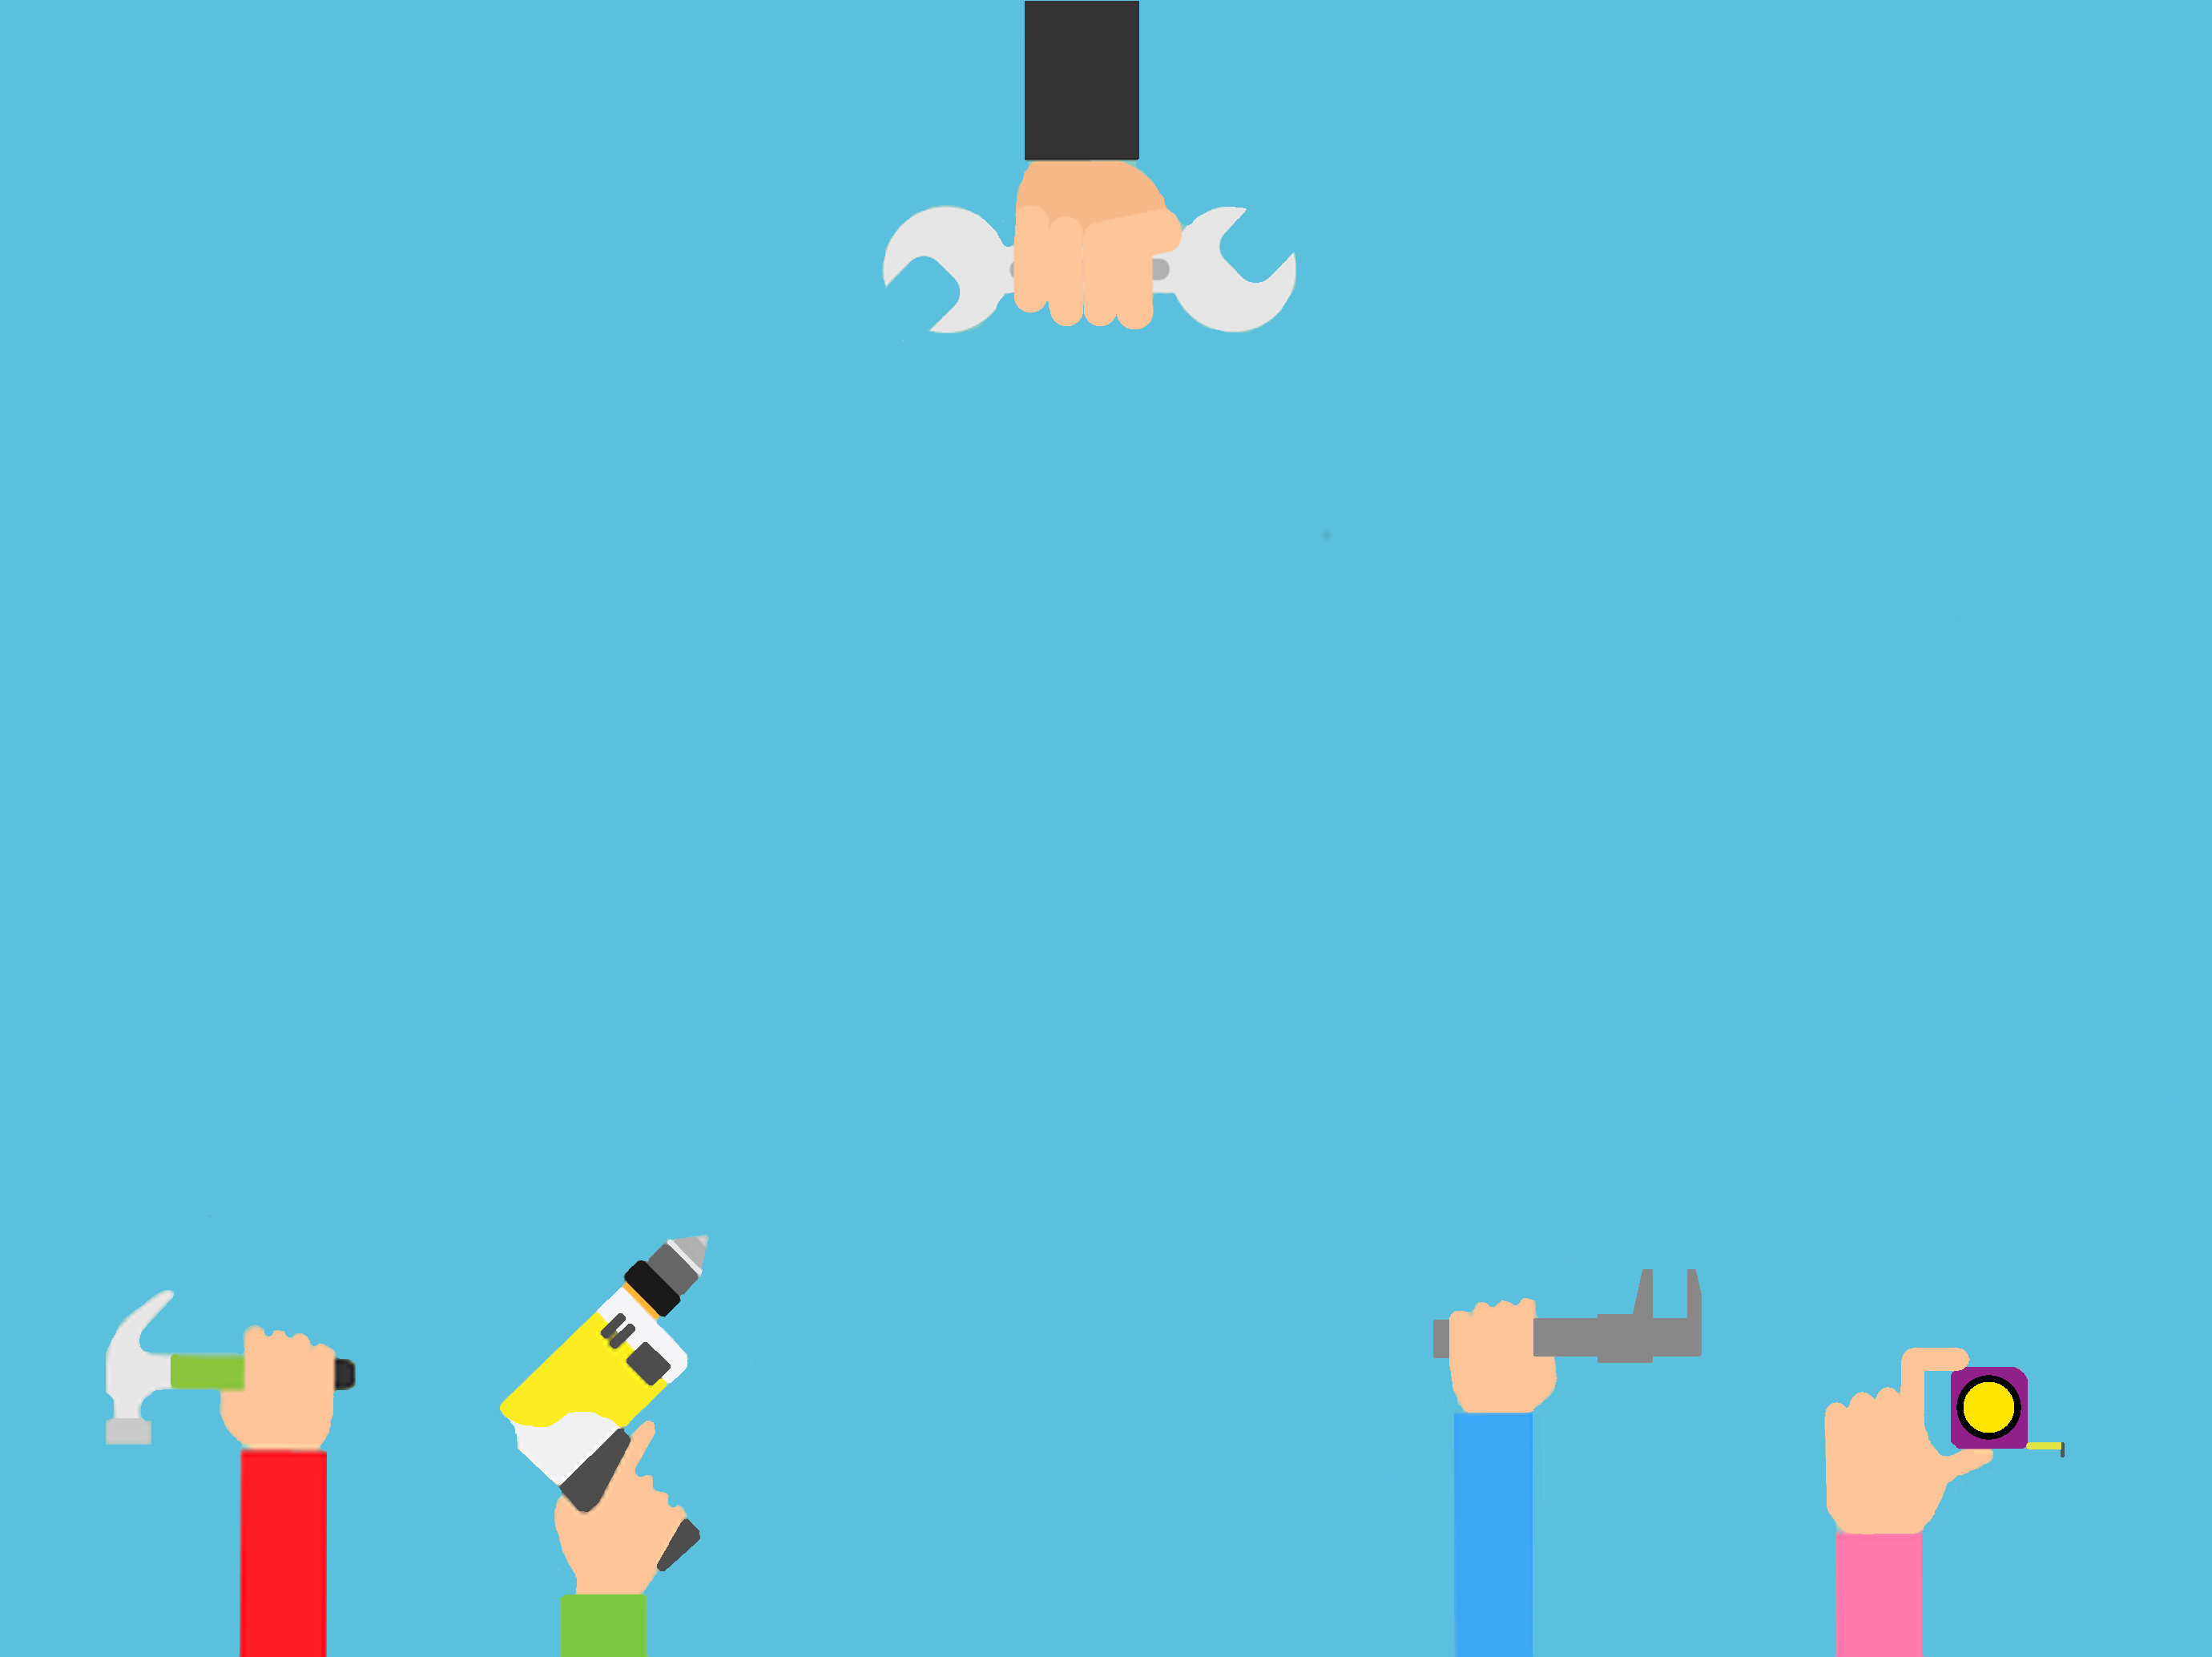
\includegraphics[width=\paperwidth]{../../img/fond}}
\frame{\titlepage}
}



\section{Écarts géométriques}

\setcounter{framenumber}{0}

{\frame{
\frametitle{Introduction}

\begin{savoir}
Vous êtes capables :
\begin{itemize}
 \item De définir le modèle nominal d'une pièce ou d'un assemblage,
 \item D'analyser un cahier des charges afin de déterminer les exigences sur une pièce.
\end{itemize}
\end{savoir}

\begin{prob}
Vous devez êtes capables :
\begin{itemize}
 \item De déterminer les défauts acceptables d'une pièce,
 \item De déterminer l'influence de ces défauts sur un assemblage.
\end{itemize}
\end{prob}
}}

{\frame{
\frametitle{Écarts géométriques: le Jeu}

\begin{defi}
Le \textbf{jeu} correspond à un espace entre des \textbf{surfaces en contact}. Il permet le mouvement mais provoque des \textbf{variations de position} relative entre ces surfaces.
\end{defi}

\textbf{Modèle} : Géométrie nominale idéale définie par le dessin d'ensemble de la solution technologique : cela définit la position idéale de l'axe.

\begin{minipage}{0.48\linewidth}
 \centering 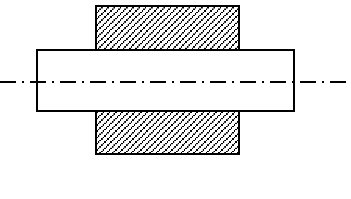
\includegraphics[width=0.5\linewidth]{img/Picture01}
\end{minipage}\hfill
\begin{minipage}{0.48\linewidth}
 \centering 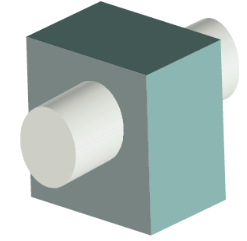
\includegraphics[width=0.3\linewidth]{img/Picture02}
\end{minipage}

\textbf{Réel} : La réalisation comporte un jeu fonctionnel radial qui permet le mouvement de rotation. Ce jeu conduit a des petits mouvements possibles non souhaités.

 \centering 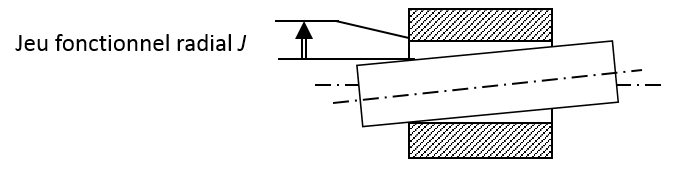
\includegraphics[width=0.5\linewidth]{img/Picture03}
}}

{\frame{
\frametitle{Écarts géométriques: les écarts}

\begin{defi}
Les \textbf{écarts} de forme et des dimensions intrinsèques des surfaces provoquent des variations de position relative entre les surfaces de contact d'une même pièce.
\end{defi}

\begin{minipage}{0.4\linewidth}
\textbf{Modèle} : Géométrie nominale idéale de l'alésage.
\end{minipage}\hfill
\begin{minipage}{0.4\linewidth}
 \centering	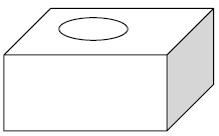
\includegraphics[width=0.5\linewidth]{img/Picture04}
\end{minipage}

\begin{minipage}{0.4\linewidth}
\textbf{Réel} : La géométrie comporte des écarts de forme et de dimension par rapport au réel.
\end{minipage}\hfill
\begin{minipage}{0.4\linewidth}
 \centering	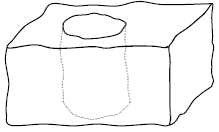
\includegraphics[width=0.5\linewidth]{img/Picture05}
\end{minipage}

Les écarts peuvent être répartis en plusieurs classes:
\begin{itemize}
 \item écarts géométriques (orientation, position, forme, état de surface,...),
 \item dimensions intrinsèques.
\end{itemize}
}}

{\frame{
\frametitle{Les torseurs de petits déplacements}

\begin{minipage}{0.6\linewidth}
\begin{rem}
Les \textbf{torseurs de petits déplacements} sont utilisés afin de déterminer la \textbf{position relative} de deux solides en fonction des \textit{écarts géométriques} entre leurs \textit{surfaces de contact}. Les grands déplacements sont écrits en majuscule.
\end{rem}
\end{minipage}\hfill
\begin{minipage}{0.3\linewidth}
 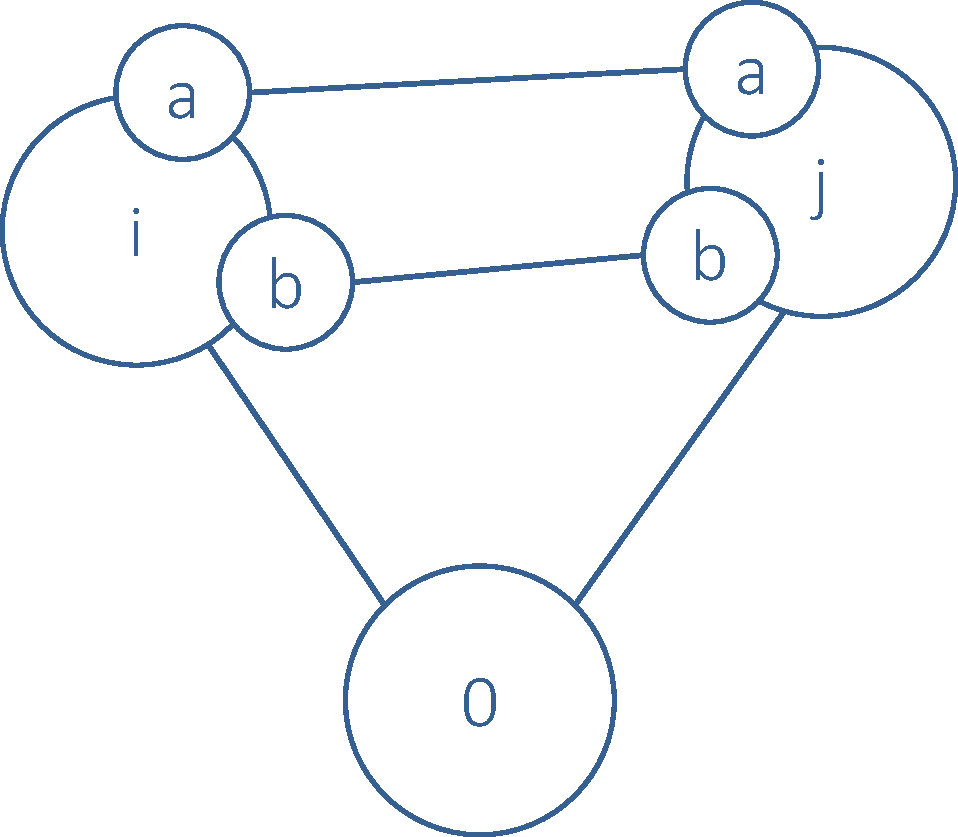
\includegraphics[width=0.8\linewidth]{img/Diag01}
\end{minipage}

\vspace{0.5cm}

\begin{minipage}{0.48\linewidth}
\begin{center}
Il existe donc un torseur jeu

$\left\{J_{iaja}\right\}=\left\{\begin{array}{c c}
\theta x_{iaja} & dx_{iaja} \\
\theta y_{iaja} & dy_{iaja} \\ \theta z_{iaja} & dz_{iaja} \end{array}\right\}_{O_1}$

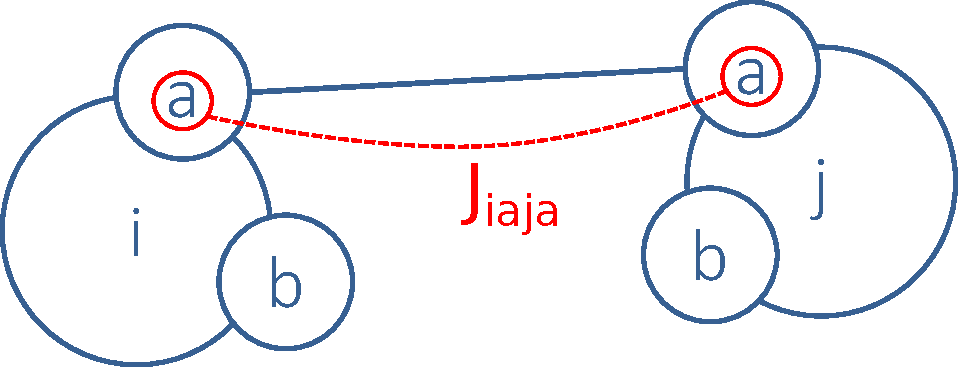
\includegraphics[height=1.5cm]{img/Diag03}
\end{center}
\end{minipage}\hfill
\begin{minipage}{0.48\linewidth}
\begin{center}
Il existe donc un torseur d'écart

$\left\{J_{iai}\right\}=\left\{\begin{array}{c c}
\theta x_{iai} & dx_{iai} \\
\theta y_{iai} & dy_{iai} \\ \theta z_{iai} & dz_{iai} \end{array}\right\}_{O_2}$

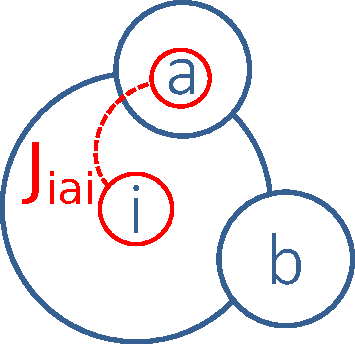
\includegraphics[height=1.5cm]{img/Diag02}
\end{center}
\end{minipage}
}}

{\frame{
\frametitle{Les torseurs de petits déplacements}

Dans l'exemple de cet assemblage, la position relative des pièces 1 et 2 peut alors être écrite comme la somme des torseurs précédents.

~\

\begin{wrapfigure}[1]{r}{5cm}
\vspace{-7mm}
\centering 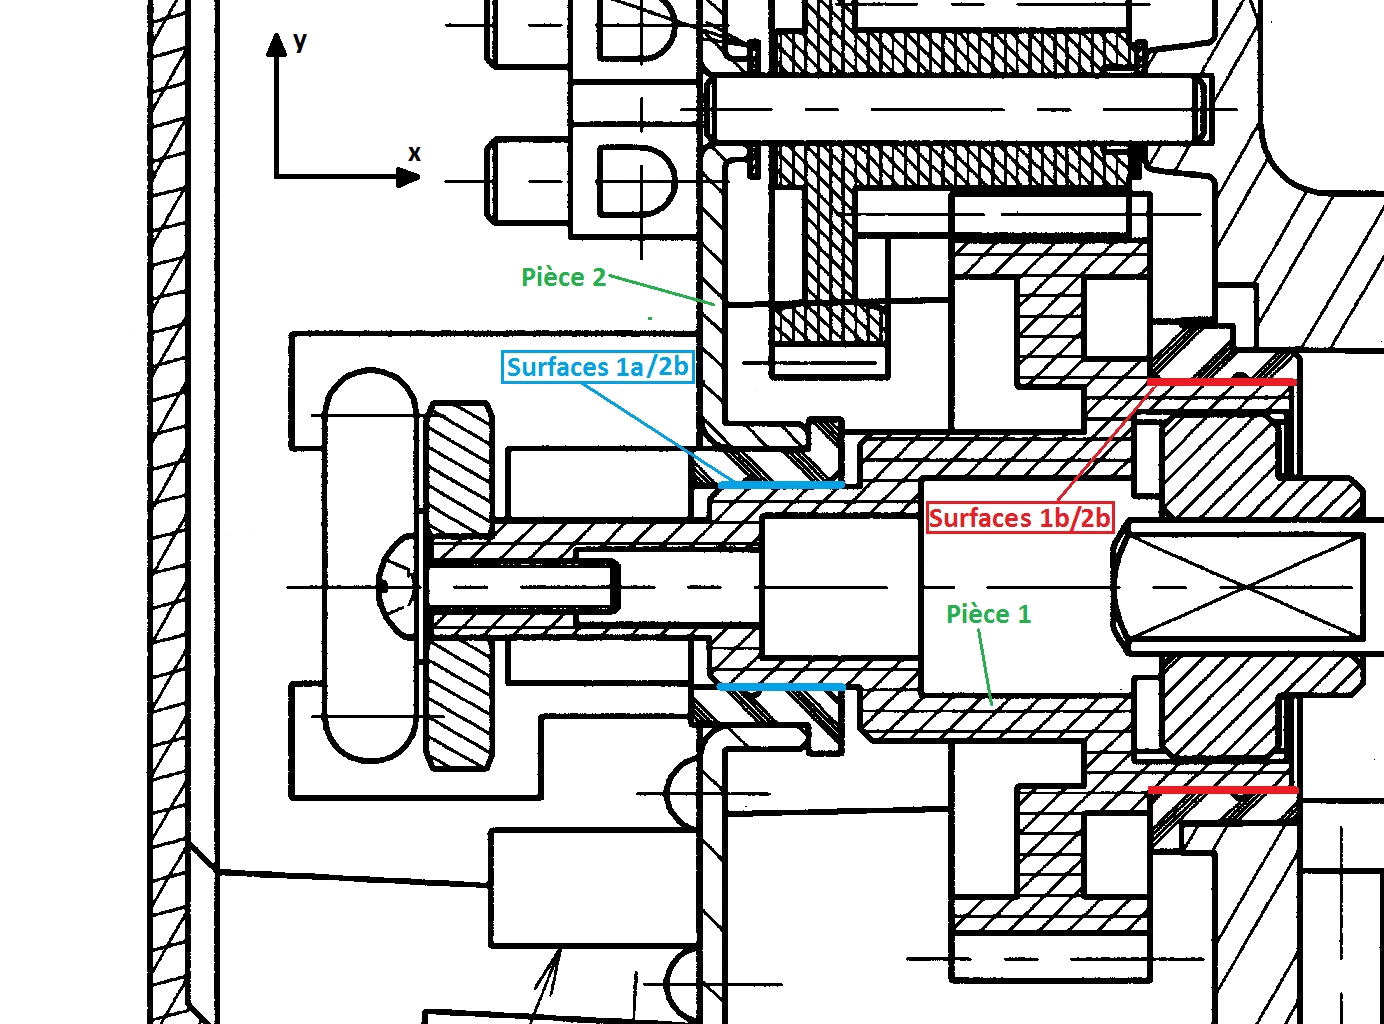
\includegraphics[width=\linewidth]{img/verin_2}
\end{wrapfigure}
$\left\{J_{21}\right\}=\left\{J_{22a}\right\}+\left\{J_{2a1a}\right\}+\left\{J_{1a1}\right\}$
$\left\{J_{21}\right\}=\left\{J_{22b}\right\}+\left\{J_{2b1b}\right\}+\left\{J_{1b1}\right\}$

$\left\{J_{22a}\right\}=\left\{\begin{array}{c c}
\Theta x_{22a} & Dx_{22a} \\
\theta y_{22a} & dy_{22a} \\
\theta z_{22a} & dz_{22a}\end{array}\right\}_{O_a}$

$\left\{\begin{array}{l}
\Theta x_{22a}+\Theta x_{2a1a}+\Theta x_{1a1}=\Theta x_{22b}+\Theta x_{2b1b}+\Theta x_{1b1} \\
\theta y_{22a}+\theta y_{2a1a}+\theta y_{1a1}=\theta y_{22b}+\theta y_{2b1b}+\theta y_{1b1} \\
\theta z_{22a}+\theta z_{2a1a}+\theta z_{1a1}=\theta z_{22b}+\theta z_{2b1b}+\theta z_{1b1} \\
Dx_{22a}+Dx_{2a1a}+Dx_{1a1}=Dx_{22b}+Dx_{2b1b}+Dx_{1b1} \\
dy_{22a}+dy_{2a1a}+dy_{1a1}=dy_{22b}-e.\theta z_{22b}+dy_{2b1b}-e.\theta z_{2b1b}+dy_{1b1}-e.\theta z_{1b1} \\
dz_{22a}+dz_{2a1a}+dz_{1a1}=dz_{22b}+e.\theta y_{22b}+dz_{2b1b}+e.\theta y_{2b1b}+dz_{1b1}+e.\theta y_{1b1}
\end{array}\right.$

}}

{\frame{
\frametitle{Analyse des équations}

Une partie des équations ne contient que des variables de \textbf{Grands Déplacements}.

$\left\{\begin{array}{l}
\Theta x_{22a}+\Theta x_{2a1a}+\Theta x_{1a1}=\Theta x_{22b}+\Theta x_{2b1b}+\Theta x_{1b1} \\
Dx_{22a}+Dx_{2a1a}+Dx_{1a1}=Dx_{22b}+Dx_{2b1b}+Dx_{1b1}
\end{array}\right.$

Une partie des équations ne contient que des variables de \textbf{Petits Déplacements}.

$\left\{\begin{array}{l}
\theta y_{22a}+\theta y_{2a1a}+\theta y_{1a1}=\theta y_{22b}+\theta y_{2b1b}+\theta y_{1b1} \\
\theta z_{22a}+\theta z_{2a1a}+\theta z_{1a1}=\theta z_{22b}+\theta z_{2b1b}+\theta z_{1b1} \\
dy_{22a}+dy_{2a1a}+dy_{1a1}=dy_{22b}-e.\theta z_{22b}+dy_{2b1b}-e.\theta z_{2b1b}+dy_{1b1}-e.\theta z_{1b1} \\
dz_{22a}+dz_{2a1a}+dz_{1a1}=dz_{22b}+e.\theta y_{22b}+dz_{2b1b}+e.\theta y_{2b1b}+dz_{1b1}+e.\theta y_{1b1}
\end{array}\right.$

Ces dernières permettent de définir des spécifications entre les surfaces en séparant les écarts et les jeux.

$\left\{\begin{array}{l}
\theta y_{2a1a}-\theta y_{2b1b}=-\theta y_{22a}-\theta y_{1a1}+\theta y_{22b}+\theta y_{1b1} \\
\theta z_{2a1a}-\theta z_{2b1b}=-\theta z_{22a}-\theta z_{1a1}+\theta z_{22b}+\theta z_{1b1} \\
dy_{2a1a}-dy_{2b1b}+e.\theta z_{2b1b}=-dy_{22a}-dy_{1a1}+dy_{22b}-e.\theta z_{22b}+dy_{1b1}-e.\theta z_{1b1} \\
dz_{2a1a}-dz_{2b1b}-e.\theta y_{2b1b}=-dz_{22a}-dz_{1a1}+dz_{22b}+e.\theta y_{22b}+dz_{1b1}+e.\theta y_{1b1}
\end{array}\right.$
}}

{\frame{
\frametitle{La spécification}

Afin de limiter les jeux ($\theta y_{2a1a}-\theta y_{2b1b}\leq \theta yj_{lim}$), il est nécessaire de limiter les écarts.

$\left\{\begin{array}{l}
-\theta y_{22a}-\theta y_{1a1}+\theta y_{22b}+\theta y_{1b1} \leq \theta y_{lim} \\
-\theta z_{22a}-\theta z_{1a1}+\theta z_{22b}+\theta z_{1b1} \leq \theta z_{lim} \\
-dy_{22a}-dy_{1a1}+dy_{22b}-e.\theta z_{22b}+dy_{1b1}-e.\theta z_{1b1} \leq d y_{lim} \\
-dz_{22a}-dz_{1a1}+dz_{22b}+e.\theta y_{22b}+dz_{1b1}+e.\theta y_{1b1} \leq d z_{lim}
\end{array}\right.$

Cela revient à imposer une spécification de parallélisme entre les deux surfaces et une spécification de position entre les deux (distance nulle).

\centering 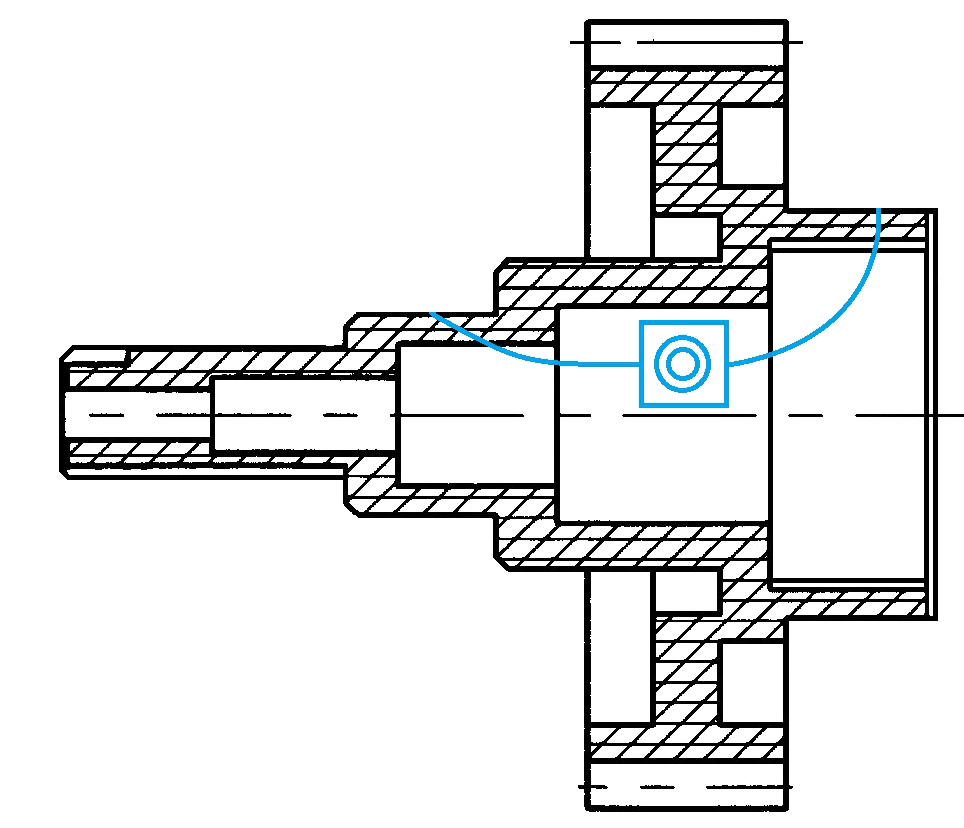
\includegraphics[width=0.4\linewidth]{img/piece}
}}

{\frame{
\frametitle{Les défauts géométriques}

\begin{savoir}
Vous devez être capables :
\begin{itemize}
 \item de déterminer les défauts potentiels d'une pièce,
 \item de modéliser l'impact de ces défauts à l'aide de torseurs de petits déplacements.
\end{itemize}
\end{savoir}

\begin{prob}

Il est nécessaire d'utiliser d'autres formes de représentation d'un mécanisme.
\begin{itemize}
 \item \textit{Problème: Comment limiter les défauts géométriques ?}
 \item \textbf{Perspectives}: Déterminer les spécifications géométriques sur une pièce.
\end{itemize}
\end{prob}

}}


\end{document}